\documentclass[12pt]{IEEEtran}
\usepackage{graphicx}
\title{\textbf{WATER MARKING}}
\author{SWATI SRI THINGBAIJAM \\swati\_t20$@$mtu.ac.in}
\date{12th Nov,2021}
\maketitle
\begin{document}
\begin{abstract}
Abstract
Digital watermarking techniques have been developed to protect the copyright of media signals. This study aims to provide a universal review and background about the watermarking definition, concept and the main contributions in this field. The study will start with a general view of digital data, the Internet and the products of these two, namely, the multimedia and the e-commerce. The study will presents an extensive and deep literature review of the field of digital watermarking and watermarking algorithms.
\end{abstract}
\section{INTRODUCTION}
Digital watermarking techniques have been developed to protect the copyright of media signals. Different watermarking schemes have been suggested for multimedia content (images, video and audio signal). This study aims to provide an extensive literature review of the multimedia copyright protection. It presents a universal review and background about the watermarking definition, concept and the main contributions in this field.\\
\centering
\begin{subfigure}{\linewidth}

\includegraphics[width=\linewidth]{flower}
\caption{WATER MARKING}
\end{subfigure}
\begin{subfigure}{\linewidth}
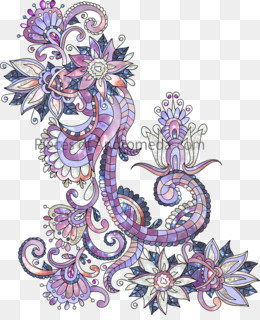
\includegraphics[width=\linewidth]{design}
\caption{WATER MARKING}
\end{subfigure}
\section{Digital Intellectual Property}
Information is becoming widely available via global networks. These connected networks allow cross-references between databases. The advent of multimedia is allowing different applications to mix sound, images, and video and to interact with large amounts of information (e.g., in e-business, distance education, and human-machine interface). The industry is investing to deliver audio, image and video data in electronic form to customers, and broadcast television companies, major corporations and photo archives are converting their content from analogue to digital form. This movement from traditional content, such as paper documents, analogue recordings, to digital media is due to several advantages of digital media over the traditional media. Some of these advantages are:
\begin{itemize}
\item The quality of digital signals is higher than that of their corresponding analogue signals. Traditional assets degrade in quality as time passes. Analogue data require expensive systems to obtain high quality copies, whereas digital data can be easily copied without loss of fidelity.
\end{itemize}\\
\begin{itemize}
\item Digital data (audio, image and video signals) can be easily transmitted over networks, for example the Internet. A large amount of multimedia data is now available to users all over the world. This expansion will continue at an even greater rate with the widening availability of advanced multimedia services like electronic commerce, advertising, interactive TV, digital libraries, and a lot more.
\end{itemize}\\

\begin{itemize}
\item Exact copies of digital data can be easily made. This is very useful but it also creates problems for the owner of valuable digital data like precious digital images. Replicas of a given piece of digital data cannot be distinguished and their origin cannot be confirmed. It is impossible to determine which piece is the original and which is the copy.
\end{itemize}\\
\begin{itemize}
\item It is possible to hide some information within digital data in such a way that data modifications are undetectable for the human senses.
\end{itemize}\\
\section{Copyright Protection of Intellectual Property}
\begin{enumerate}
\item An important factor that slows down the growth of multimedia-networked services is that authors, publishers and providers of multimedia data are reluctant to allow the distribution of their documents in a networked environment. This is because the ease of reproducing digital data in their exact original form is likely to encourage copyright violation, data misappropriation and abuse. These are the problems of theft and distribution of intellectual property. Therefore, creators and distributors of digital data are actively seeking reliable solutions to the problems associated with copyright protection of multimedia data.\\

\item Moreover, the future development of networked multimedia systems, in particular on open networks like the Internet, is conditioned by the development of efficient methods to protect data owners against unauthorized copying and redistribution of the material put on the network. This will guarantee that their rights are protected and their assets properly managed. Copyright protection of multimedia data has been accomplished by means of cryptography algorithms to provide control over data access and to make data unreadable to non-authorized users. However, encryption systems do not completely solve the problem, because once encryption is removed there is no more control on the dissemination of data. The concept of digital watermarking arose while trying to solve problems related to the copyright of intellectual property in digital media. It is used as a means to identify the owner or distributor of digital data. Watermarking is the process of encoding hidden copyright information since it is possible today to hide information messages within digital audio, video, images and texts, by taking into account the limitations of the human audio and visual systems.
\end{enumerate}
\centering
\begin{subfigure}{\linewidth}

\includegraphics[width=\linewidth]{china rose}
\caption{Fig : DRAWING }
\end{subfigure}
\begin{subfigure}{\linewidth}
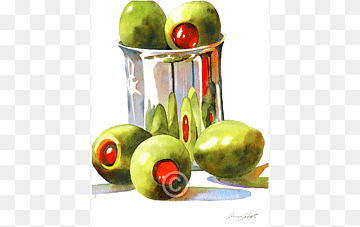
\includegraphics[width=\linewidth]{fruit}
\caption{Fig : FRUIT}
\end{subfigure}\\
\section*{Digital Watermarking: What, Why, When and How?}
It seems that digital watermarking is a good way to protect intellectual property from illegal copying. It provides a means of embedding a message in a piece of digital data without destroying its value. Digital watermarking embeds a known message in a piece of digital data as a means of identifying the rightful owner of the data. These techniques can be used on many types of digital data including still imagery, movies, and music.
\section{What is Digital Watermarking?}
\begin{enumerate}
\item A digital watermark is a signal permanently embedded into digital data (audio, images, video, and text) that can be detected or extracted later by means of computing operations in order to make assertions about the data. The watermark is hidden in the host data in such a way that it is inseparable from the data and so that it is resistant to many operations not degrading the host document. Thus by means of watermarking, the work is still accessible but permanently marked.

\item Digital watermarking techniques derive from steganography, which means covered writing (from the Greek words stegano or “covered” and graphos or “to write”). Steganography is the science of communicating information while hiding the existence of the communication. The goal of steganography is to hide an information message inside harmless messages in such a way that it is not possible even to detect that there is a secret message present. Both steganography and watermarking belong to a category of information hiding, but the objectives and conditions for the two techniques are just the opposite. In watermarking, for example, the important information is the “external” data (e.g., images, voices, etc.). The “internal” data (e.g., watermark) are additional data for protecting the external data and to prove ownership. In steganography, however, the external data (referred to as a vessel, container, or dummy data) are not very important. They are just a carrier of the important information. The internal data are the most important. On the other hand, watermarking is not like encryption. Watermarking does not restrict access to the data while encryption has the aim of making messages unintelligible to any unauthorized persons who might intercept them. Once encrypted data is decrypted, the media is no longer protected. A watermark is designed to permanently reside in the host data. If the ownership of a digital work is in question, the information can be extracted to completely characterize the owner.

\item Digital watermarking is an enabling technology for e-commerce strategies: conditional and user-specific access to services and resources. Digital watermarking offers several advantages. The details of a good digital watermarking algorithm can be made public knowledge. Digital watermarking provides the owner of a piece of digital data the means to mark the data invisibly. The mark could be used to serialize a piece of data as it is sold or used as a method to mark a valuable image. For example, this marking allows an owner to safely post an image for viewing but legally provides an embedded copyright to prohibit others from posting the same image. Watermarks and attacks on watermarks are two sides of the same coin. The goal of both is to preserve the value of the digital data. However, the goal of a watermark is to be robust enough to resist attack but not at the expense of altering the value of the data being protected. On the other hand, the goal of the attack is to remove the watermark without destroying the value of the protected data. The contents of the image can be marked without visible loss of value or dependence on specific formats. For example a bitmap (BMP) image can be compressed to a JPEG image. The result is an image that requires less storage space but cannot be distinguished from the original.
\section*{When Did the Technique Originate?}
The idea of hiding data in another media is very old, as described in the case of steganography. Nevertheless, the term digital watermarking first appeared in 1993, when Tirkel et al. (1993) presented two techniques to hide data in images. These methods were based on modifications to the least significant bit (LSB) of the pixel values.\\
\section{Discrete Cosine Transform-Based Digital Watermarking}
Several watermarking algorithms have been proposed to utilize the DCT. However, the Cox et al. (1995, 1997) and the Koch and Zhao (1995) algorithms are the most well-known DCT-based algorithms. Cox et al. (1995) proposed the most well-known spread spectrum watermarking schemes. Figure 3 shows the block diagram of the Cox algorithm. The image is first subjected to a global DCT. Then, the 1,000 largest coefficients in the DCT domain are selected for watermarking. They used a Gaussian sequence of pseudo-random real numbers of length 1,000 as a watermark. This approach achieves good robustness against compression and other common signal processing attacks. This is a result of the selection of perceptually significant transform domain coefficients. However, the algorithm is in a weak position against the invariability attack proposed by Craver (1997). Also, the global DCT employed on the image is computationally expensive.

\section{Watermarking Standardization Issue}
\begin{itemize}
\item The most important question about watermarking technology is whether watermarking will be standardized and used in the near future. There are several movements to standardize watermarking technology, but no one standard has prevailed at this moment in time. Some researchers have been working to develop a standardized framework for protecting digital images and other multimedia content through technology built into media files and corresponding application software. However, they have lacked a clear vision of what the framework should be or how it would be used.\\

\item In addition, there was a discussion about how and whether watermarking should form part of the standard during the standardization process of JPEG2000. The requirements regarding security have been identified in the framework of JPEG2000. However, there has been neither in-depth clarification nor a harmonized effort to address watermarking issues. It is important to deduce what really needs to be standardized for including the watermarking concept in JPEG2000 and to what extent. The initial drafts of the JPEG2000 standard did not mention the issue of watermarking. However, there is a plan to examine how watermarking might be best applied within JPEG2000. The features of a given watermarking scheme are likely to offer designers an opportunity to integrate watermarking technology into JPEG2000 for different application such as distributing images on the Internet. Also, standardization of digital watermarking will influence the progress in imaging standards of JPEG2000 where the data security will be part of this standard. Therefore, the likelihood is that watermarking technology will be used in conjunction with JPEG2000 (Clark, 2000).
\end{itemize}
\section{CONCLUSION}
This study was started with a general view of digital data, the Internet and the products of these two, namely, multimedia and e-commerce. It provided some initial background and history of digital watermarking. This study gave an extensive and deep literature review of the field of digital watermarking. The concept of digital watermarking and the requirements of digital watermarking were discussed and digital watermarking algorithms were reviewed. They were grouped into three main collections based on the embedding domain, that is, spatial domain techniques, transform domain techniques or feature domain techniques. The algorithm of the frequency domain were further subdivided into wavelet, DCT and fractal transform techniques. Finally, the future perspective of digital watermarking was highlighted.\\ \\ \\ \\
\\ \\
\textbf{REFERENCE}
\begin{enumerate}
\item IJ Cox, ML Miller, JA Bloom, C Honsinger - 2002 - Springer\\
\item CI Podilchuk, W Zeng - IEEE Journal on selected areas in …, 1998 - ieeexplore.ieee.org\\
\item F Cayre, C Fontaine, T Furon - IEEE Transactions on signal …, 2005 - ieeexplore.ieee.org\\
\item VM Potdar, S Han, E Chang - INDIN'05. 2005 3rd IEEE …, 2005 - ieeexplore.ieee.org\\
\item FAP Petitcolas - IEEE signal processing magazine, 2000 - ieeexplore.ieee.org\\
\end{enumerate}
\end{document}